\chapter{Analisi di Contesto e definizione di Challenge}

In questo capitolo viene introdotta una definzione formalizzata di Challenge, successivamente alla quale viene introdotta un'analisi di contesto, necessaria per la definizione di attori e come essi interagiscono tra loro.

\section{Challenge}
Viene definita \textbf{Challenge} una sfida proposta dall'azienda esterna all'università ed è composta da:

\begin{itemize}
    \item Nome della Challenge.
    \item Laboratorio nel quale si svolgerà.
    \item Descrizione accurata del problema da risolvere.
    \item Data di inizio. 
    \item Data di fine.
    \item Orario.
    \item Autore, ossia il nome dell'azienda.
    \item Descrizione testuale del premio messo in palio dall'azienda per il gruppo vincitore.
    \item Limite temporale per l'iscrizione dei gruppi.
    \item Dimensione di ogni gruppo. 
    \item Numero massimo di gruppi.
\end{itemize}

Ogni azienda può formare più di una Challenge. Vi possono essere molteplici Challenge all'interno di un laboratorio.

Alla conclusione del limite temporale previsto l'azienda che ha creato la Challenge \textbf{deve} selezionare i gruppi che parteciperanno entro un quantitativo di giorni. Gli utenti facenti parte dei gruppi selezionati riceveranno una mail contenente i dati della Challenge con eventuali dettagli aggiuntivi.

Alla conclusione di una Challenge ad ogni studente è richiesto di compilare un form per fornire feedback sull'attività appena svolta per poterlo inviare all'azienda.
L'applicativo non prevede uno strumento di comunicazione tra azienda e studente oltre al form sopracitato.

Vi è una diretta correlazione \textbf{l'area tematica} della challenge proposta dall'azienda ed il \textbf{laboratorio didattico}, in quanto la suddetta può formalizzare una challenge di una specifica area tematica solamente nel laboratorio corrispondente.

Alla creazione della Challenge, essa viene inserita in un Pending state finchè non viene accettata/rifiutata dal moderatore. Dopo tale azione essa entra in uno stato Accettato o Rifiutato in base alla scelta del suddetto.

\section{Attori}
Di seguito vengono riportati gli attori dell'applicativo. Ad ogni attore vengono associati i requisiti funzionali correlati sulla base delle azioni che possono effettuare.

\subsection{Studente}
Uno studente viene definito come una persona iscritta all'Università di Trento e che attualmente ricopre il ruolo di studente del corso di laurea triennale o magistrale, dottorando o ricercatore.

Tale utente può effettuare le seguenti azioni:

\begin{itemize}
    \item Selezionare le aree tematiche al quale è interessato per poter ricevere notifiche alla validazione di nuove Challenge da parte del moderatore.
        \begin{itemize}
            \item Lo studente può decidere di non ricevere email inerenti a nuove Challenge facente parte della sua area tematica.
        \end{itemize}
    \item Visualizzare la lista delle Challenges facenti parte dell'area di interesse selezionata.
    \item Visualizzare informazioni inerenti alla Challenge selezionata.
    \item Iscriversi alla Challenge formando o entrando a far parte di un gruppo.
    \item Al termine di una Challenge lo studente può compilare un form per fornire un feedback all'azienda sulla Challenge appena compiuta. 
    \item Al termine di una Challenge lo studente può visualizzare il feedback ricevuto da parte del Company Manager.
\end{itemize}

Uno studente può avere molteplici aree di interesse e può partecipare a più di una Challenge appartenente al suo settore di interesse.

\subsection{Gruppo di Studenti}
Per poter partecipare ad una Challenge gli studenti devono formare un gruppo. Un gruppo è definito da uno o più studenti ed un Tutor. 
Alla formazione di un nuovo gruppo il primo nominativo diviene il capogruppo ed ad esso viene richiesto di:
 \begin{enumerate}
        \item Fornire il nome per il gruppo.
        \item Selezionare il Tutor del gruppo. 
        \item Fornire una presentazione testuale del gruppo. 
\end{enumerate}

Alla formazione di un gruppo esso è in stato di \textbf{Pending}. Esso può cambiare di stato quando:
\begin{itemize}
    \item Il tutor selezionato visualizza il dettaglio del gruppo ed accetta di farne parte. In tal caso lo stato del gruppo diviene \textbf{Tutored}. 
    \item Il tutor selezionato visualizza il dettaglio del gruppo e rifiura di farna parte. In tal caso lo stato del gruppo diviene \textbf{Rejected}. 
    \item Il Company Manager visualizza il dettaglio del gruppo e lo accetta per partecipare alla Challenge. In tal caso lo stato del gruppo diviene \textbf{Accepted}. 
    \item Il Company Manager visualizza il dettaglio del gruppo e lo rifiuta. In tal caso lo stato del gruppo diviene \textbf{Rejected}. 
\end{itemize}

Per partecipare ad una Challenge è richiesto che il gruppo sia in \textbf{Accepted} state. Il gruppo ha un tempo di vita limitato alla durata della Challenge, dunque tale entità viene creata per la Challenge.



\subsection{Moderatore}
Tale figura é incaricata di accettare le Challenges che potranno essere effettuate, oltre al modificare i membri dei gruppi. Ogni Laboratorio ha un solo responsabile. Esso viene riferito anche come \textit{responsabile di laboratorio}.

L'utente può effettuare le seguenti azioni:
\begin{itemize}
    \item Visualizzare tutti i laboratori che gestisce. 
    \item Visualizzare tutte le challenge proposte per quel laboratorio.
    \item Accettare o rifiutare le Challenges proposte dall'azienda.
    \item Prenotare il laboratorio nel caso la Challenge venga accettata. Tale azione è esterna all'applicativo.
    \item Gestire gli account delle aziende(creazione, eliminazione, modifica, etc). Tale azione è esterna all'applicativo.
\end{itemize}


\subsection{Company Manager}

Questo utente viene creato all'interno del Sistema in seguito alla formulazione ed approvazione di una richiesta esterna all'applicativo.

Tale utente può effettuare le seguenti azioni:
\begin{itemize}
    \item Creare una Challenge.
    \item Visualizzare tutte le Challenge che ha effettuato.
    \item Modificare Challenge non accettate o rifiutate.
    \item Accedere al dettaglio della Challenge e visualizzare ogni gruppo.
    \item Accettare o rifiutare l'ingresso di un gruppo ad una determinata Challenge. 
    \item Al termine di una Challenge il Company Manager può fornire il feedback mediante un modulo apposito per il lavoro svolto ad ogni gruppo e studente. 
    \item Al termine di una Challenge il Company Manager può Visualizzare il feedback di tutti gli studenti che hanno partecipato alla Challenge e lo hanno fornito.
\end{itemize}

\subsection{Tutor}
Tale figura è un membro del DISI ed è incaricata della supervisione di un gruppo durante una Challenge. Alla creazione di un gruppo per partecipare ad una Challenge \textbf{deve} essere selezionato. 

Esso può svolgere le seguenti attività:
\begin{itemize}
    \item Visualizzare tutti i gruppi che hanno richiesto la sua partecipazione. 
    \item Accettare di entrare a far parte di un gruppo o rifiutarlo. Si ricordi che all'accettazione da parte del tutor il gruppo entra in \textbf{Tutored }state. 
\end{itemize}

\section{Diagramma di Contesto}

Nel seguente elenco è posisbile trovare una descrizione ad alto livello delle relazioni tra le differenti componente esterne al sistema. Bisogna notare che tale rappresentazione viene effettuata a livello logico e non è correlata all'architettura del framework utilizzato.

Il \textbf{Company Manager} è un \textbf{attore} e può svolgere le seguenti azioni: può effettuare il login, gestire le proprie challenge, accettare o rifiutare i gruppi (già in tutored state, ossia gruppi i quali siano già formati ed accettati da un Tutor), oltre a poter compilare e visualizzare i feedback inerenti alle challenge dell'azienda.

Il \textbf{Moderatore} è un \textbf{attore} e può svolgere le seguenti azioni: può visualizzare i laboratori che modera, accedere al loro dettaglio ed accettare o rifiutare le Challenge proposte per il laboratorio.

Lo \textbf{Studente} è un \textbf{attore} e può svolgere le seguenti azioni: può cambiare i propri interessi in modo da vedere solo le challenge che facciano parte della sua area di interesse, può decidere se essere aggiornato o meno sulle nuove Challenge approvate dal moderatore, formare e gestire i gruppi creati appositamente per le Challenge, fornire e visualizzare i feedback relativi alle Challenge effettuate. 

Il \textbf{Tutor} è un \textbf{attore} e può svolgere le seguenti azioni: può visualizzare i gruppi che hanno richiesto la sua partecipazione, accettare o rifiutare di farne parte.

Il \textbf{Sistema di invio mail/notifica} è un \textbf{subordinato} ed è l'infrastruttura che permette l'invio di email nei seguenti casi ed ai seguenti attori:
\begin{itemize}
    \item Creazione di una nuova Challenge da parte del Company Manager : viene inviata una mail a tutti i moderatori del laboratorio nella quale la Challenge deve essere svolta. 
    \item Accettazione o rifiuto di una Challenge da parte del Moderatore: viene inviata una mail al Company Manager che ha creato la Challenge, oltre che ad una mail a tutti gli studenti che hanno richiesto di essere aggiornati sulle nuove Challenge e i quali interessi siano un super-set della Challenge accettata.
    \item Creazione di un nuovo gruppo da parte di uno studente : viene inviata una mail al Tutor selezionato dal capogruppo.
    \item Accettazione o rifiuto di entrare a far parte di un gruppo da parte del Tutor : viene inviata una mail a tutti i membri del gruppo.
    \item Accettazione o rifiuto di un gruppo da parte del Company Manager : viene inviata una mail a tutti i membri del gruppo.
\end{itemize}

\textbf{Shibboleth} è un \textbf{subordinato} ed è il modulo che permette di effettuare il login all'interno dell'applicativo. Esso è un software open source che permette l'autenticazione federata e single sign-on.

Il \textbf{Database} è un \textbf{subordinato} ed è il corrispettivo di ciò che è stato definito come componente Model all'interno dell'architettura di Django. Esso gestisce le transazioni con il Database ed è l'unico modulo in grado di accedere ai dati. Esso permette la traduzione di query da linguaggio python al linguaggio della base di dati selezionata. 

Di seguito viene riportato il diagramma di contesto dell'applicativo.


\begin{figure}[H]
    \centering
    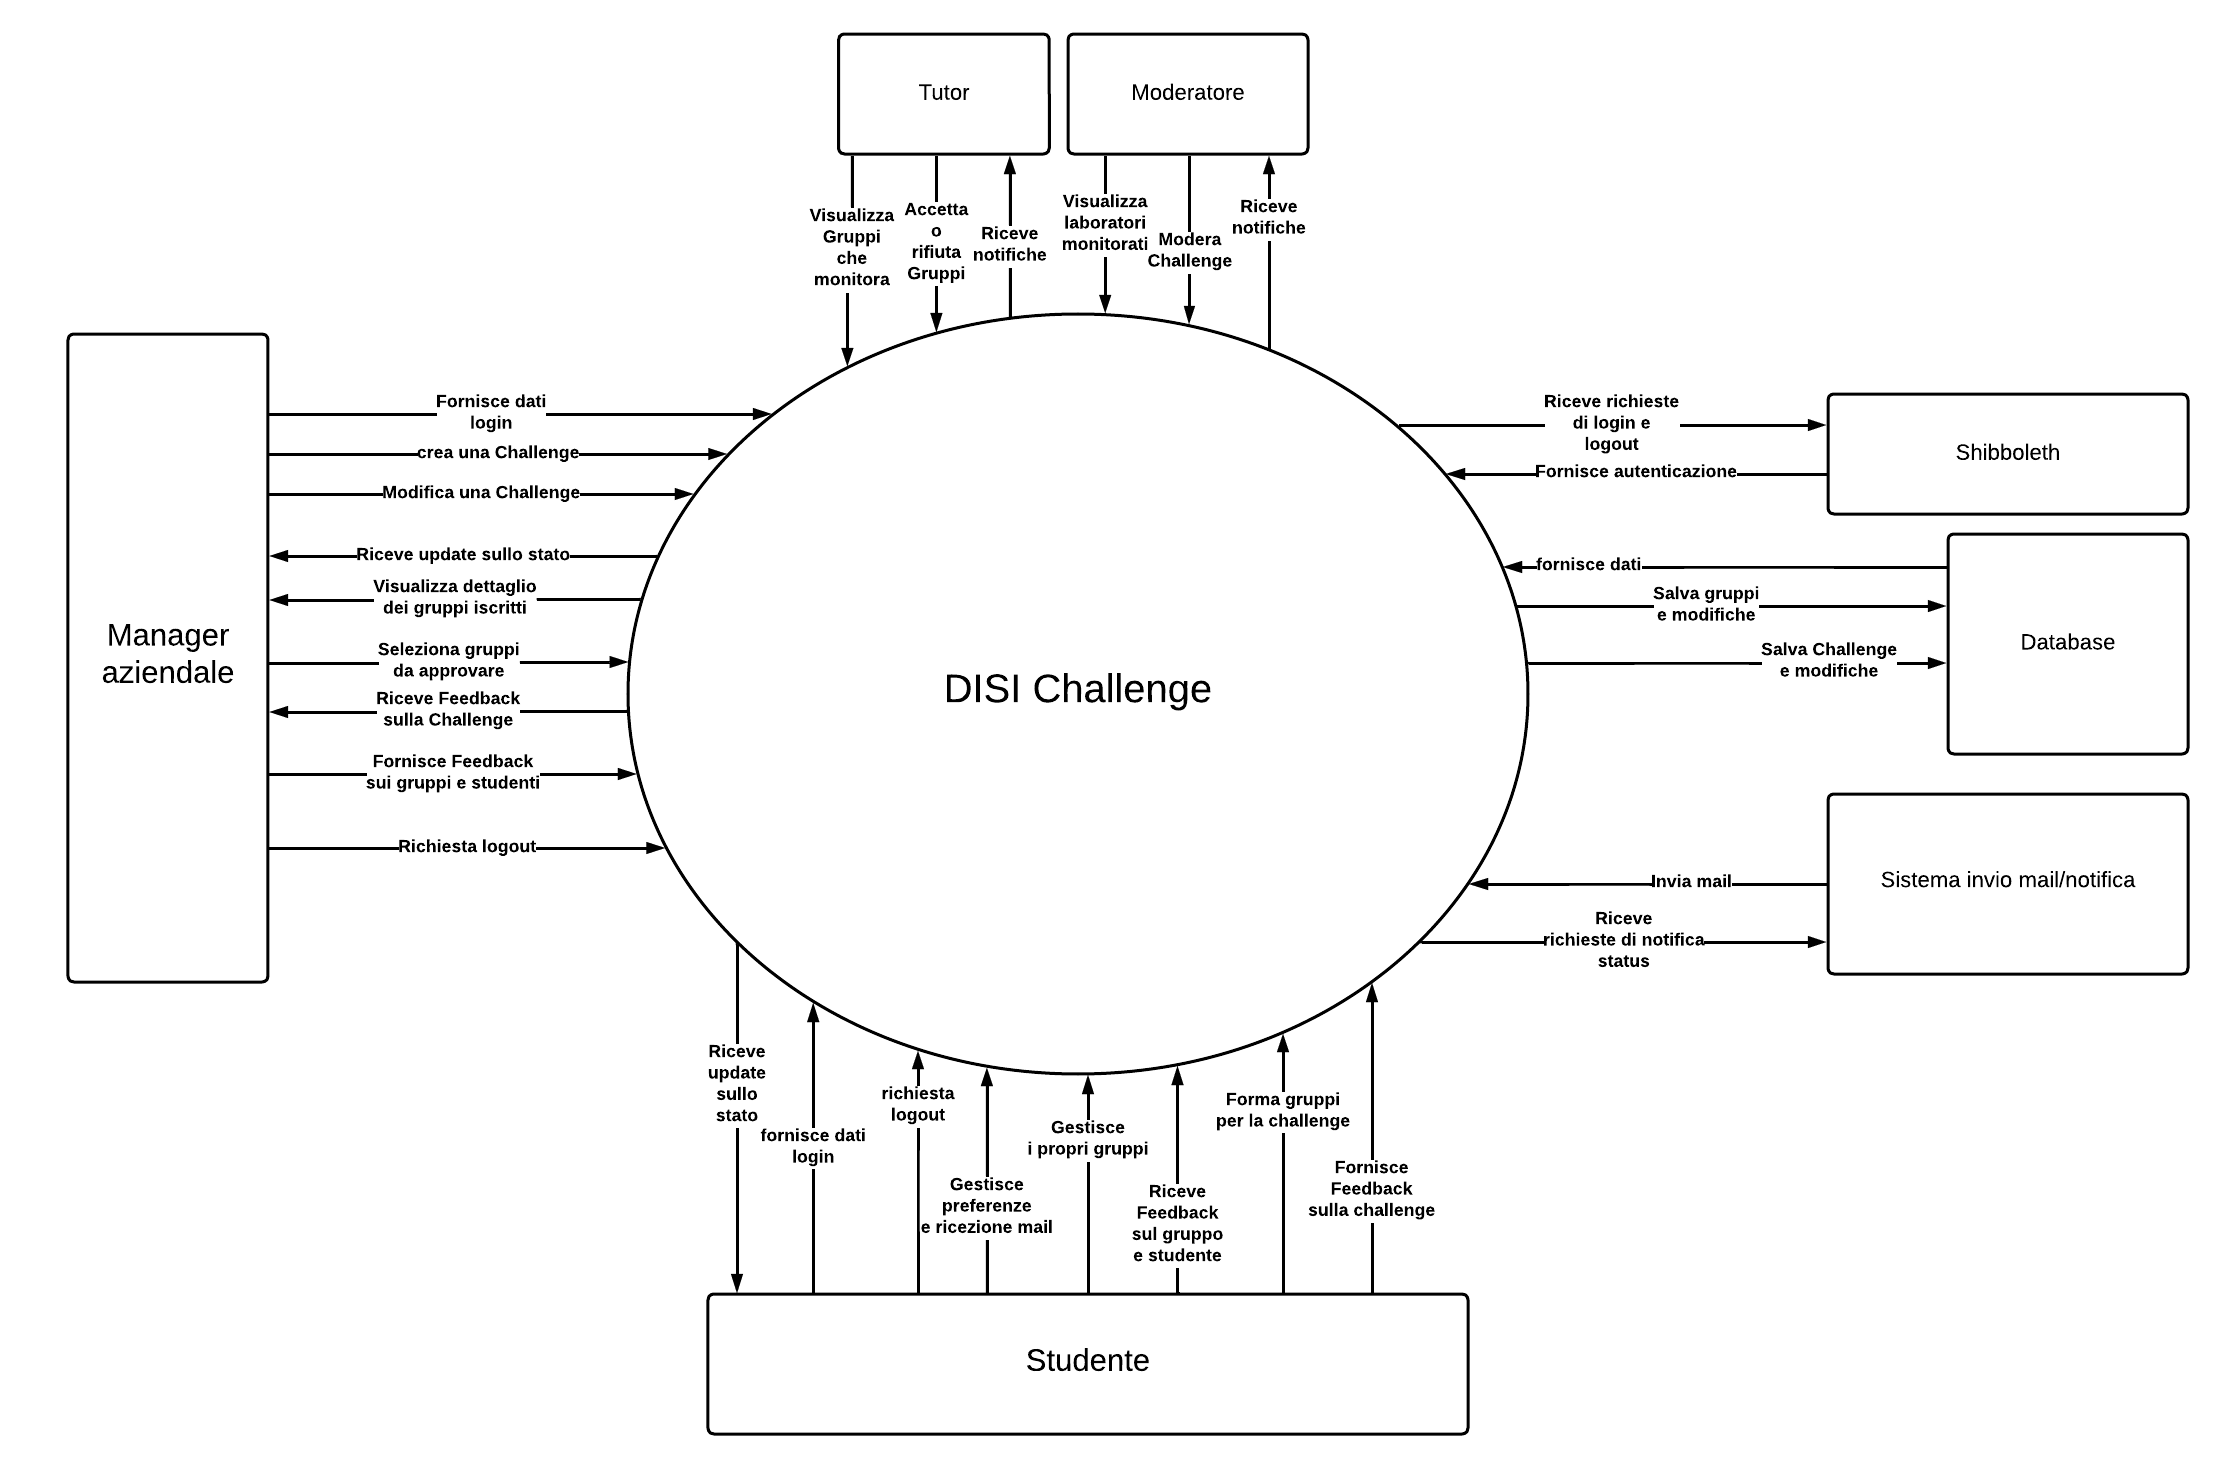
\includegraphics[scale=0.46]{images/diagrama_di_contesto.png}
    \label{fig:diagrama_di_contesto}
    \caption{Diagramma di contesto}
\end{figure}

\section{Processo di creazione e partecipazione ad una Challenge}

Data la complessità del processo, viene di seguito utilizzato un diagramma Business Process Model Notation (BPMN) per descrivere il processo di creazione e partecipazione ad una Challenge. 

\begin{figure}[H]
    \centering
        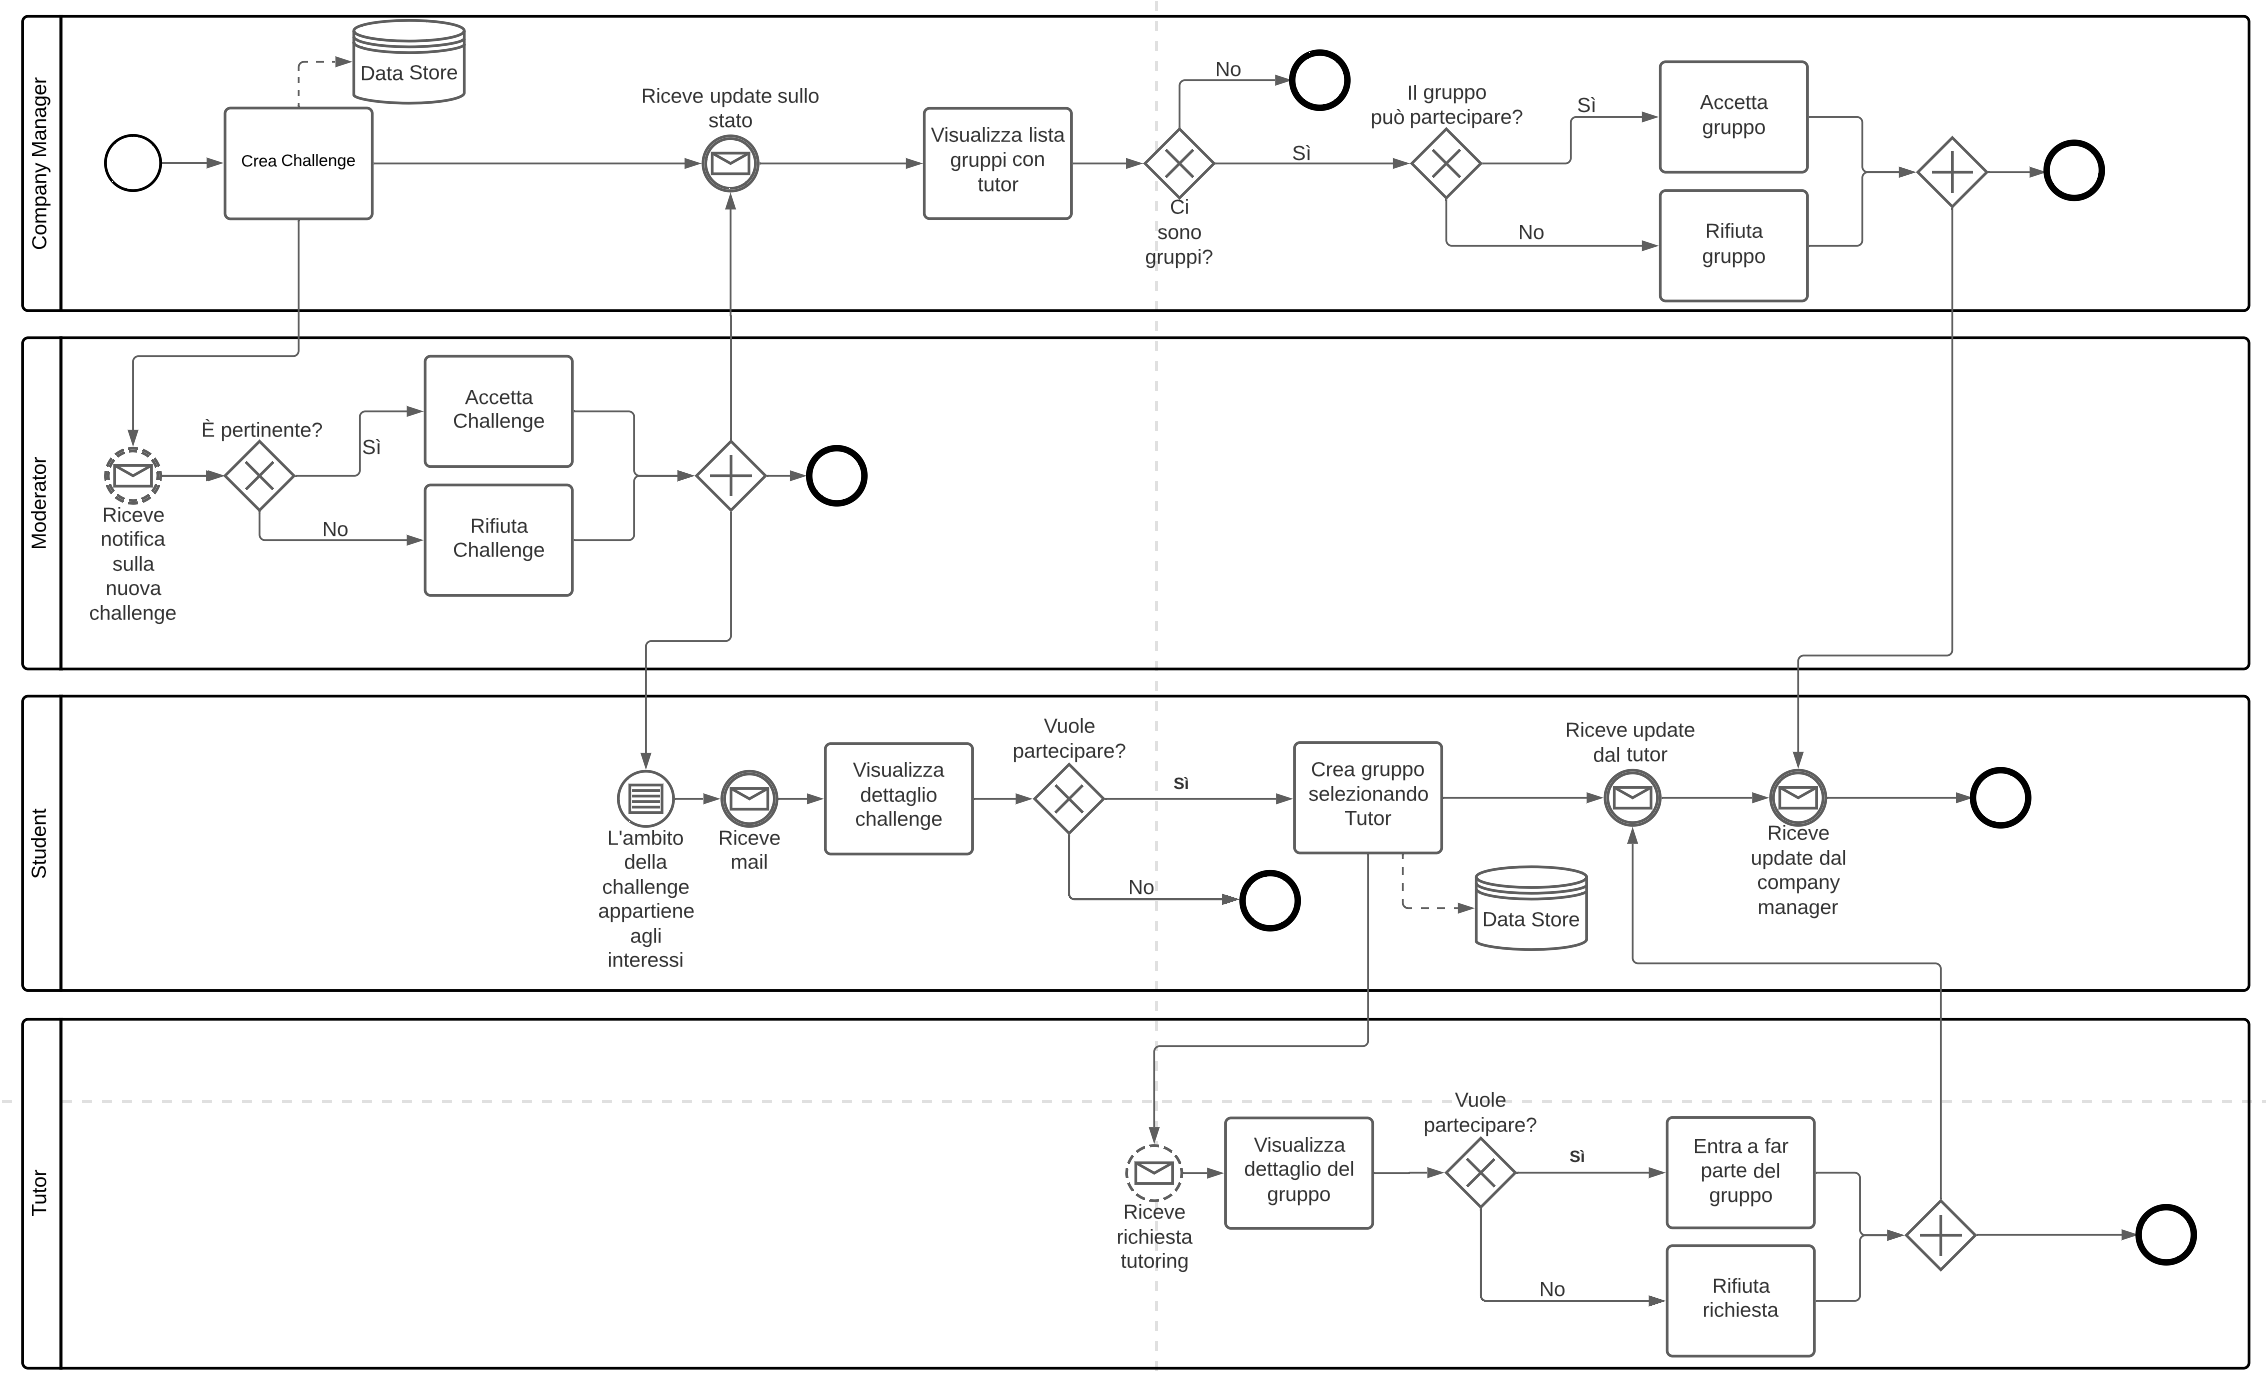
\includegraphics[width=0.95\textwidth]{images/BPMN_Challenge.png}
    \caption{BPMN della creazione di una Challenge}
    \label{fig:BPMN_Challenge}
\end{figure}


Il flow dell'applicativo è il seguente:
\begin{enumerate}
    \item Il Company Manager crea una Challenge ed una mail viene inviata ai moderatori del laboratorio scelto come luogo per svolgere la Challenge.
    \item Il Moderatore riceve la mail di richiesta di accettazione di una Challenge. Accede alla sua area personale, dove può visualizzare i suoi laboratori ed accede al dettaglio della Challenge. Alla conferma o rifiuto della Challenge viene inviata una email al Company Manager ed agli studenti che hanno sia scelto di essere aggiornati sulle nuove Challenge, sia che abbiano interessi che siano un super-set della Challenge accettata.
    \item Gli studenti possono visualizzare la challenge approvata e formare dei gruppi o entrare a far parte di gruppi già creati mediante il codice fornito al capo gruppo. Alla creazione di un gruppo il tutor selezionato riceve una email.
    \item Il tutor riceve la email e può accettare o rifiutare di entrare a far parte del gruppo. Alla sua decisione viene inviata una mail a tutti i membri del gruppo.
    \item Il Company Manager può accedere al dettaglio della Challenge ed accettare o rifiutare di far partecipare i gruppi che sono già stati accettati da un tutor. Alla sua decisione viene inviata una mail a tutti i membri del gruppo.
\end{enumerate}


\section{Valutazione delle Challenge e dei gruppi}

Al termine di una Challenge, agli attori 
\clearpage
